\begin{figure}[H]
  \centering
  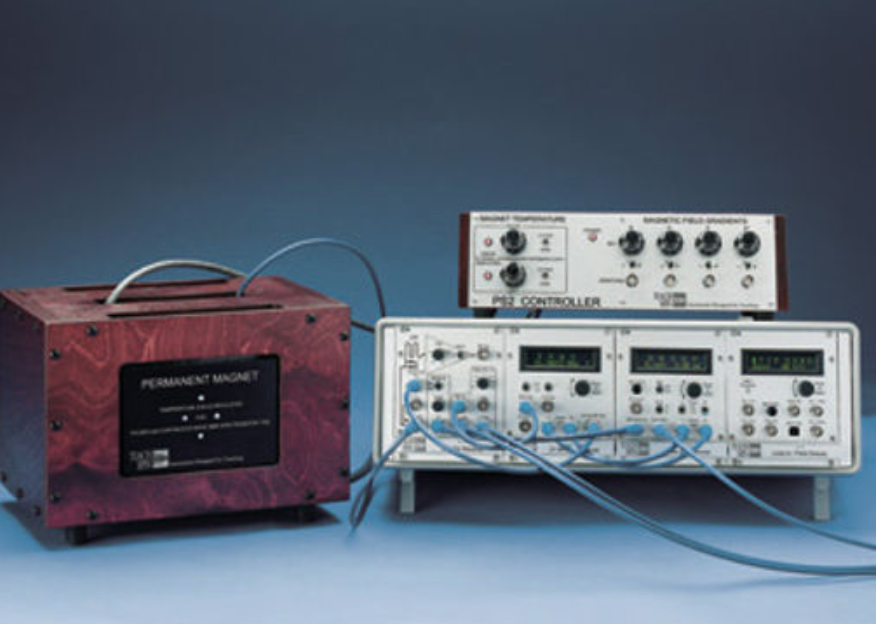
\includegraphics[scale=0.5]{resources/aufbau.png}
  \caption{Abbildung des Versuchsaufbaus \cite{skizze}}
  \label{fig:aufbau}
\end{figure}
\noindent Die Abbildung \ref{fig:aufbau} zeigt den experimentellen Aufbau des
Versuchs zur Kernspinresonanz. Auf der linken Seite befindet sich ein
Permanentmagnet mit eingelassener Bohrung. In dieser befindet sich eine Spule,
in deren Inneres die Probe deponiert werden kann. Durch die Anordnung der Probe
im Permanentmagneten wird das Magnetfeld am Ort der Probe als homogen angesehen.
Die rechts im Bild befindlichen Steuergeräte dienen zur Einstellung der
Schwingungsfrequenz und Schwingungsphase, der Pulslänge und Anzahl an Pulsen, zur Bestimmung
der Periodendauer, sowie zur Einstellung der Parameter der Shims-Spulen. Ein
Oszilloskop (nicht im Bild) wird zum Export der
Daten und zur Justage genutzt. Zusätzlich steht noch ein Thermometer zur
Bestimmung der Temperatur am Ort der Probe bereit.
